\chapter{文件与文件管理}
\label{files-and-file-management}

\begin{intro}
  在这一部分,我们将重新介绍你可能所不知道的「文件」以及「文件」的管理,以及一些实用的文件管理的技巧。
  看完这一部分,你将可以找到下面这些问题的答案:
  \begin{itemize}
    \item 为什么很多人说「不建议把文件放在桌面上」?
    \item C 盘总是「红了」,为什么?为什么有人建议把软件装到 D 盘里?
    \item 「扩展名」是什么?「打开方式」又是什么?为什么有时候我电脑上的 Word 文档就打不开了?
  \end{itemize}
\end{intro}

如上一章所言,硬盘是电脑中存放数据的地方,而「文件」则是数据存放的具体形式。
你所撰写的 Word 文档、制作的 PPT 幻灯片、从网上下载的图片,乃至各个 app 或者说软件本身,都以文件的形式存储在硬盘上。

这一部分,我们将具体介绍「文件」和文件的管理。
这是《Missing》需要动手实践的第一章,也是我们合理、有效地使用电脑的第一课。

\section{硬盘的分区}

打开桌面上的【此电脑】(但其实打开的东西叫「文件资源管理器」),我们往往可以看到多于一个的「盘」,例如 C 盘、D 盘等。
这样的「盘」学名叫做「分区」,顾名思义,它们是将硬盘上的空间人为地划分成了一些子空间。

\begin{figure}[htb!]
  \centering
  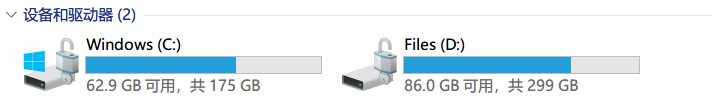
\includegraphics[width=13cm]{assets/Hans_Disks.jpg}
  \caption{Hans 电脑上的分区}
  \label{Hans_Disks}
\end{figure}

例如,上图是 Hans 的笔记本电脑「此电脑」中的分区。
可以看到,这两个分区一个大小为 175 GB,另一个大小为 299 GB,相加为 474 GB——这是这台电脑的硬盘可用总空间。

划分分区的意义,在于帮助我们更好地管理文件。
分区划分之后,各个分区之间就仿佛被「隔离」开来了,如图 \ref{Disk_Parts} 所展示的那样。
即使我们「格式化」一个分区(这样会删除这个分区中的所有文件),也不会影响另外一个分区里面的文件。

\begin{figure}[htb!]
  \centering
  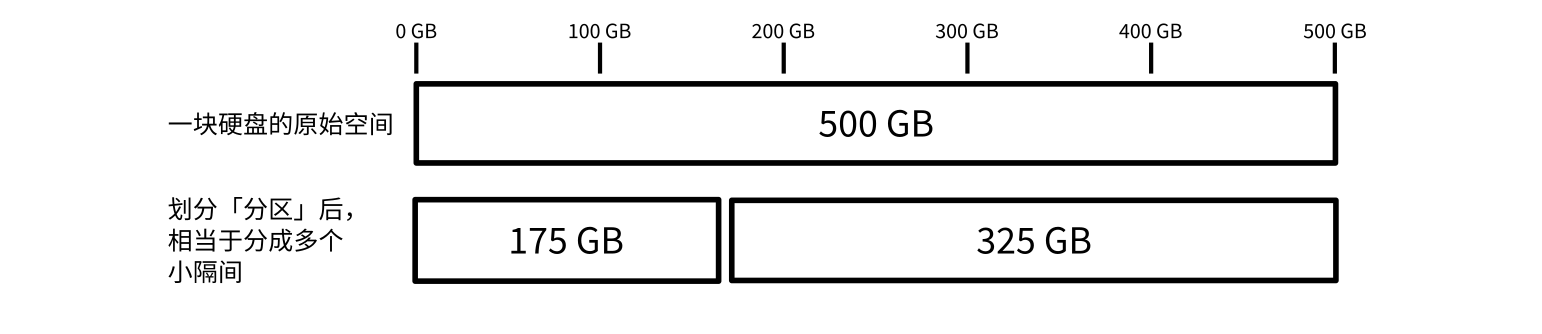
\includegraphics[width=.9\textwidth]{assets/Disk_Parts.png}
  \caption{硬盘与分区的关系}
  \label{Disk_Parts}
\end{figure}

在 Windows 系统中,分区会被给予两个标识符,或者说「名字」:

\begin{itemize}
  \item 一个是「\regcolor{盘符}」,盘符是一个英文字母加上冒号 \verb|:| 构成的。
    我们所称呼的「C 盘」「D 盘」正是指盘符中的那个字母。
    如上图,左方分区的盘符是 \verb|C:| ,右方分区的盘符是 \verb|D:| 。
    盘符一般在被指定之后就不方便更换了。在今天,Windows 系统中的盘符都是从字母 C 开始\footnote{这是因为 A 和 B 两个盘符在过去是留给「软盘」的,但软盘早就已经成为历史了,不过这个习惯却保留了下来。}的。
  \item 另一个是「\regcolor{卷标}」,这是一个可选的标识符,它是一定长度的文本。
    在上图中,C 盘的卷标是「Windows」,D 盘的卷标是「Files」。
    盘符的作用是让系统和软件识别分区,而卷标的作用是帮助我们用户更加直观地了解分区的作用,因而卷标是可以随时更换的。
    事实上,通过右键某一分区,选择【重命名】,就可以更换卷标了。如果你什么都不写,它默认叫做「本地磁盘」。
\end{itemize}

\begin{figure}[htb!]
  \centering
  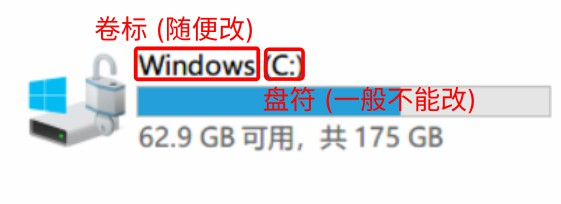
\includegraphics[width=7cm]{assets/Volume_Name_and_Letter.jpg}
  \caption{盘符与卷标}
  \label{Volume_Name_and_Letter}
\end{figure}

我们在\nameref{computer-and-its-components}中提到,操作系统本身也是一个大软件,那么这个软件放在硬盘上的哪呢?
对于 Windows 而言,整个 Windows 系统默认放在 C 盘里。
双击打开电脑 C 盘,你会看到一些你可能不熟悉的文件夹,例如 \verb|Windows| 文件夹,Windows 系统自己的许多文件就存在其中。

也许你听过「不要把软件安装到 C 盘」这样的说法。这是有根据的。
系统本身就已经很庞大,系统自身工作产生的一些文件也会被自动地放在 C 盘内,导致 C 盘本身空间就容易变得局促。
如果还将大量的软件装在 C 盘,会让 C 盘更加「不堪重负」,结果就是——红了。

在本章的后续部分,以及\nameref{software-installation}中,我们会详细介绍,怎样把我们的软件以及其他东西放在 C 盘以外的地方,以及这样做的其他好处。

\section{文件、文件名和文件类型}

「文件」是数据存储在硬盘上的形式。这么说可能有些抽象,直观地说,文件就是我们每天都打交道的东西:

\begin{figure}[htb!]
  \centering
  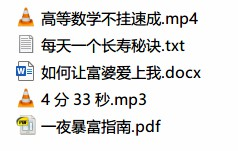
\includegraphics[width=7cm]{assets/Files.jpg}
  \caption{一些文件}
  \label{Files}
\end{figure}

文件有自己的「名字」,称为「文件名」。
在 Windows 系统中,文件名可以分成三个部分:

\begin{itemize}
  \item 「主名」是指文件名中,点号 \verb|.| 之前的部分。
    这部分内容可以自定,相当于人类的姓名。
    上图中,「 \verb|如何让富婆爱上我| 」和「 \verb|一夜暴富指南| 」等都是文件的主名。
  \item 「点号」是指文件名中间的那个「 \verb|.| 」。
  \item 「扩展名」是指文件名中,点号「 \verb|.| 」之后的部分\footnote{有时候我们称呼文件的扩展名时也会把点号包含进去。下面两种说法是等价的:
      \begin{itemize}
        \item 某文件的扩展名是\texttt{txt}。
        \item 某文件的扩展名是\texttt{.txt}。
      \end{itemize}}。
    扩展名展示着文件的类型,它会告诉操作系统,这个文件应该用什么方式来打开。
    例如,上图中「 \verb|每天一个长寿秘诀.txt| 」中的「 \verb|txt| 」就是这个文件的扩展名,它说明这个文件是一个「文本文档」,应该使用「记事本」打开。
\end{itemize}

\begin{figure}[htb!]
  \centering
  \begin{minipage}{.48\textwidth}
    \centering
    
\includegraphics[width=.95\textwidth]{assets/File_Name.png}
    \caption{文件名结构}
    \label{File_Name}
  \end{minipage}
  \begin{minipage}{.48\textwidth}
    \centering
    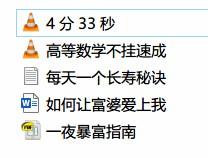
\includegraphics[width=.95\textwidth]{assets/Files_No_Ext.jpg}
    \caption{没有显示扩展名的文件}
    \label{File_No_Ext}
  \end{minipage}
\end{figure}

扩展名也是可以人为改变的,但这样往往会出问题——试想,对于上图中的 \texttt{高等数学不挂速成.mp4} ,它本来是一个 \verb|mp4| 文件,即「视频文件」,应该用看视频的软件打开。
如果你强行把它改成 \verb|txt| ,系统就会用「记事本」来打开一个「视频文件」——用错误的工具打开文件。

如果你的电脑上,文件的扩展名没有被显示(也就是说你只能看到文件的主名),如图 \ref{File_No_Ext} 所示。
在 Windows 10 中请点选文件夹窗口上方的【查看】选项卡,然后勾选【文件扩展名】,如图 \ref{Windows_10_set_full_filename} 所示;在 Windows 11 中请点选文件夹窗口上方的【查看】菜单,然后勾选【显示】→【文件扩展名】,如图 \ref{Windows_11_set_full_filename} 所示。

\begin{figure}[htb!]
  \centering
  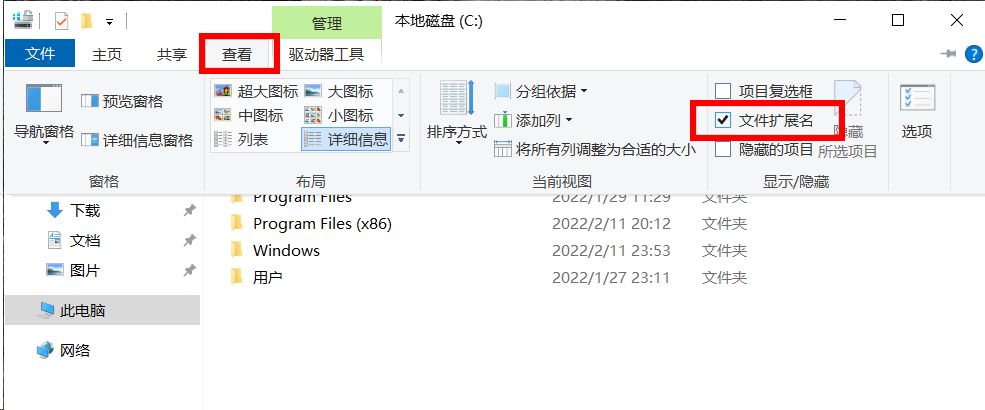
\includegraphics[width=10cm]{assets/Windows_10_set_full_filename.png}
  \caption{Windows 10 设置方法}
  \label{Windows_10_set_full_filename}
\end{figure}

\begin{figure}[htb!]
  \centering
  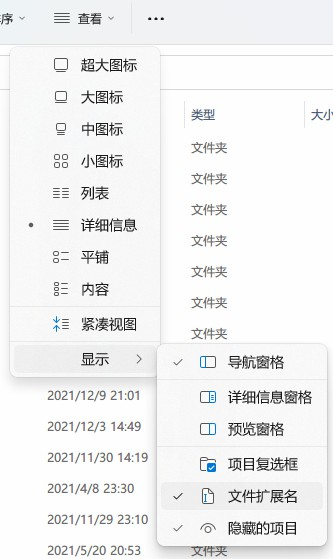
\includegraphics[width=4cm]{assets/Windows_11_set_full_filename.jpg}
  \caption{Windows 11 设置方法}
  \label{Windows_11_set_full_filename}
\end{figure}

在打开这个选项之后,文件扩展名不仅是可见的,甚至是可以改变的——但如上文所说,扩展名不能随便改,因为改了之后系统就会用错误的工具去打开它。
右键某一文件,选择【重命名】,你会看到系统会自动帮你选中文件的「主名」,而不选中「扩展名」。
如果你执意更改文件的「扩展名」,系统会发出一个提示:

\begin{figure}[htb!]
  \centering
  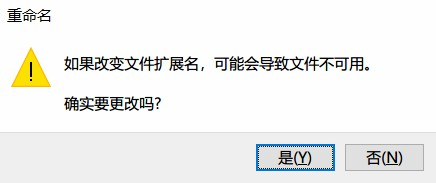
\includegraphics[width=6cm]{assets/Warning_of_Changing_Ext.jpg}
  \caption{尝试更改扩展名……}
  \label{Warning_of_Changing_Ext}
\end{figure}

「那既然这样,我不想不小心突然间改掉文件的扩展名,还不如不开呢。」如果你有这样的想法,那么另一重危险正悄然降临。且看下面的两个文件:

\begin{figure}[htb!]
  \centering
  \begin{minipage}{.48\textwidth}
    \centering
    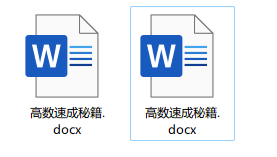
\includegraphics[width=.95\textwidth]{assets/fake_doc.png}
    \caption{两个神奇的文件}
    \label{fake_doc}
  \end{minipage}
  \begin{minipage}{.48\textwidth}
    \centering
    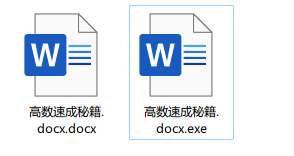
\includegraphics[width=.95\textwidth]{assets/fake_doc_revealed.png}
    \caption{揭示扩展名后}
    \label{fake_doc_revealed}
  \end{minipage}
\end{figure}

这两个「高数速成秘籍」看起来完全一样,就是两个正常的 Word 文档,但众所周知,一个目录下不可能存在两个文件名相同的文件,显然这里面必然有猫腻。
现在打开文件扩展名,这两个文件的名称变成了下面这个样子,可见,其中一个居然是可执行文件(\verb|exe|)格式,即一个应用程序(详见下文),只是图标故意被做成了 Word 文档的样子。
所以,看不到扩展名的话,指不定哪天有居心叵测的人发来一个这样伪装的病毒,那可就不好了。


\section{文件夹、路径和目录}

「文件夹」是一个用来存放其他文件的结构。
不妨想象一下现实中的「文件夹」:

\begin{figure}[htb!]
  \centering
  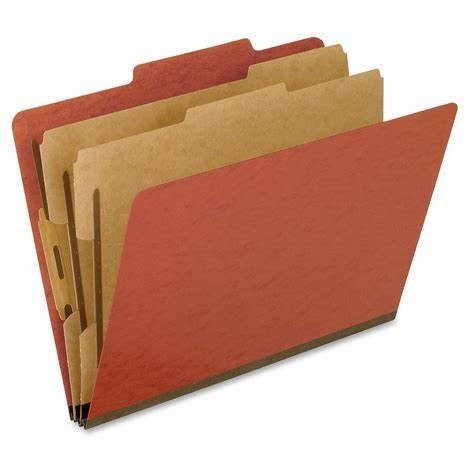
\includegraphics[width=4cm]{assets/Real_Folder.jpg}
  \caption{真实的文件夹}
  \label{Real_Folder}
\end{figure}

在这样的一个「文件夹」中,可以放很多各类「文件」。
而电脑中的文件夹除了能放文件之外,还可以放很多的「子文件夹」,即「文件夹里面的文件夹」。
这个过程可以循环重复,因而一个文件夹的内部结构可以相当错综复杂。

如果抽象地把整个电脑看成一个巨大的「文件夹」,那么不同的分区就是这个巨大「文件夹」之下的几个子文件夹,我们的某一份文件就是在这些子文件夹之下的某一个角落里。
假设在 D 盘的 \verb|missing| 文件夹之中有一个叫做 \verb|源文件| 的子文件夹,在这个子文件夹中有一个文件叫 \verb|第三章.docx| ,我们用这种方式表示这个 \verb|第三章.docx| 文件在整个电脑中的位置:

\begin{verbatim}
  D:\missing\源文件\第三章.docx
\end{verbatim}

这一长串东西表示出 \verb|第三章.docx| 这个文件在电脑中的具体位置,我们把一长串东西称为 \verb|第三章.docx| 这个文件的「路径」(严格来说叫做「绝对路径」)。
不难发现,路径是从「分区」(也就是「盘」)开始,用反斜杠 \verb|\| 作为分隔,一级一级文件夹地展开,最后到具体的文件。
类似的,不只是文件,文件夹的路径也可以用这样的方式来表示,例如

\begin{verbatim}
  D:\missing\源文件
\end{verbatim}

表示的就是 \verb|源文件| 这个文件夹在电脑中的位置。
一个文件 / 文件夹的「路径」是唯一确定的;一个「路径」也能唯一确定一个文件 / 文件夹。

也许你有听说过「目录」这个名字。其实「目录」就是文件夹。
例如这个说法「打开目录 \verb|D:\missing\public\| 」 指的就是打开 D 盘中 \verb|missing| 文件夹里的 \verb|public| 文件夹。

目录(文件夹)一层一层的结构可以像图 \ref{Catalog_Tree} 一样从上到下画出来,称作「目录树」。
在目录树这种形式中,文件夹之间是「上下级」的关系,故「文件 A 在文件夹 B 中」也可以称作「文件 A 在文件夹 B 下」或者「A 在目录 B 下」甚至是「A 在 B 下」。
也就是说,「下」这个字就是「在……里」的意思。

\begin{figure}[htb!]
  \centering
  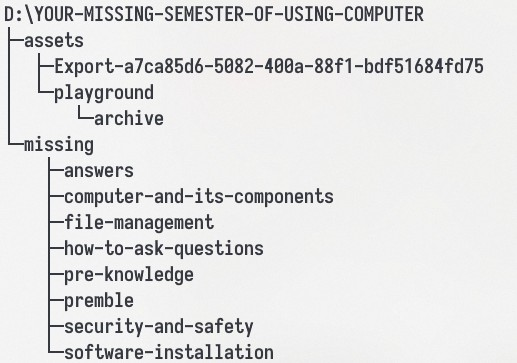
\includegraphics[width=8cm]{assets/Catalog_Tree.jpg}
  \caption{目录树}
  \label{Catalog_Tree}
\end{figure}

借助目录树这样的结构,我们就能理解「根目录」这个概念了。
一个盘的「根目录」指的是这个盘之下的第一级目录(恰好是目录「树」的「根」),例如 C 盘根目录就指的是路径 \verb|C:\| 。

\section{程序本身——可执行文件(\texttt{exe}文件)}

这一节我们介绍一种类型特殊的文件——「可执行文件」。
我们提到,数据是以文件的形式存储在硬盘上的,比如你所撰写的 Word 文档,它们都存储成了扩展名为 \verb|doc| 或者 \verb|docx| 的文件;
你所下载的图片,它们的扩展名则往往是 \verb|jpg| 、 \verb|jpg| 或者 \verb|gif| 。
而我们又提到,软件或者说 app 也是以文件的形式存储在硬盘上的。
那么,软件本身是什么格式的文件呢?

一个软件的核心是一个或多个「程序」,而程序是以「可执行文件」的形式存储的。
\regcolor{普通的文件,需要用其他的某个软件才能正常打开;而「可执行文件」双击就能运行自身,这就是「可执行」(Executable)的意思。}

可执行文件的扩展名是 \verb|exe| 。
对于这种类型的文件,系统不会想着用别的软件去打开它,而是直接运行它自身。
可执行文件有时被直接称为「程序文件」或者「程序」。

需要注意的是,电脑上的一款软件(或者说 app,在《Missing》中我们会同时使用这两种称呼)可能不仅仅只有一个程序,也就不止一个可执行文件。
下面是软件「网易云音乐」所在的文件夹中的一部分:

\begin{figure}[htb!]
  \centering
  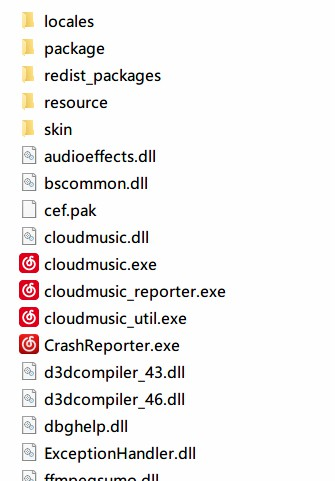
\includegraphics[width=5cm]{assets/NetEase_Music.jpg}
  \caption{网易云音乐的目录}
  \label{NetEase_Music}
\end{figure}

可以看到,「网易云音乐」这个 app 有着这些文件:

\begin{itemize}
  \item 可执行文件 \verb|cloudmusic.exe| ,这个是 app 的主体,即「网易云音乐」的主程序。
  \item 可执行文件 \verb|cloudmusic_reporter.exe| , \verb|cloudmusic_util.exe| 等。
    这些文件是 app 运行时的其他辅助程序,可以想象成乐队中主唱身边的吉他手 / 键盘手 / 鼓手 / 伴舞等。
    它们往往无法单独运行,而 \verb|cloudmusic.exe| 这个主文件脱离它们也不能运行。
  \item 一大堆的 \verb|dll| 和其他格式的文件。这些是 app 工作时不可或缺的依赖文件。
  \item 一些子文件夹,存储着 app 运行需要的另外一些东西。
\end{itemize}

每次我们启动「网易云音乐」,运行的都是 \verb|cloudmusic.exe| 这个可执行文件。
然而,这个文件的运行离不开放在它边上的那一堆辅助文件——如果你把 \verb|cloudmusic.exe| 复制到另外的一个地方,双击运行,大概率会直接报错;即使不报错,功能也必然有不正常。

在下一章我们在介绍软件的安装时会继续说明这个问题。

\section{文件的「替身」——快捷方式}

\begin{figure}[htb!]
  \centering
  
\includegraphics[width=10cm]{assets/Shortcut.png}
  \caption{快捷方式}
  \label{Shortcut}
\end{figure}

你是怎么启动「网易云音乐」的呢?

一般来说,我们会双击桌面上的「网易云音乐」或者点击开始菜单中的「网易云音乐」。
不管是桌面上的「网易云音乐」还是开始菜单里的「网易云音乐」,它们都是不是这个 app 本身——app 本身的样子我们在上面刚刚看过——而是另一种特殊类型的文件,称作「快捷方式」。

\begin{wrapfigure}[12]{r}{6cm}
  \centering
  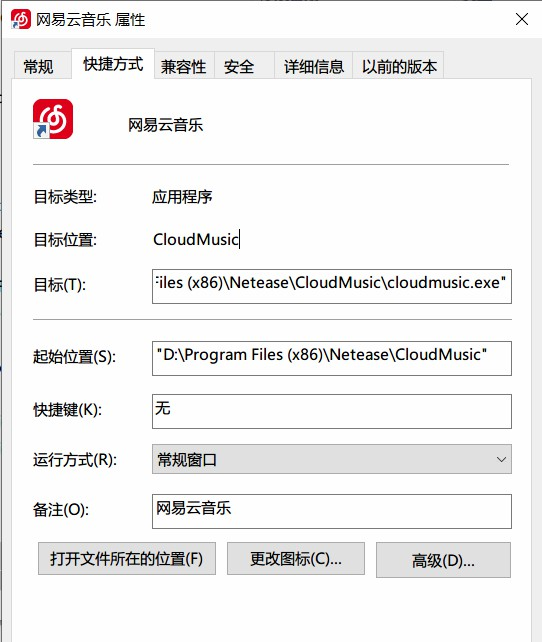
\includegraphics[width=5cm]{assets/NetEase_Music_Link.jpg}
  \caption{桌面上的「网易云音乐」}
  \label{NetEase_Music_Link}
\end{wrapfigure}

「快捷方式」可以看成某个具体文件的单向「指针」或者说「替身」,指向电脑某个角落里的某个文件。
它的扩展名是 \verb|lnk| ,但实际上不可见\footnote{千万不要手动把一个正常文件的扩展名改成\texttt{lnk},否则就很难改回来了。}。
你桌面上的「网易云音乐」,指向的正是网易云音乐软件目录下的那个 \verb|cloudmusic.exe| 文件。右击桌面上的【网易云音乐】,选择【属性】,会弹出这个快捷方式的详细信息:

其中「目标」一栏填写的正是 \verb|cloudmusic.exe| 这个可执行文件,即「网易云音乐」的主程序的路径:

\begin{verbatim}
  D:\Program Files (x86)\Netease\CloudMusic
  \cloudmusic.exe
\end{verbatim}

因此,你双击打开这个「网易云音乐」快捷方式,就会打开 \verb|cloudmusic.exe| 这个文件。
如果你\regcolor{删掉了这个快捷方式,它并不会影响 \texttt{cloudmusic.exe} 这个文件,不会影响你电脑上安装的网易云音乐本身。}

\begin{note}
  因此,卸载软件的方式可不是把桌面上的「快捷方式」删掉就完事的。
\end{note}

所有类型的文件以及文件夹都可以制作出无数个快捷方式。
如果你想给自己的某个文件 / 文件夹制作一个快捷方式,只需右键它,选择【发送到】→【桌面快捷方式】,就能在桌面生成一个指向这个文件的快捷方式了。
这个快捷方式可以挪到系统的任何地方,也可以复制粘贴出很多个副本。它们全都指向原来的那个文件本身。

一般来说,快捷方式的图标左下角会有一个「↗」符号。
这个符号标志着这个文件并非某文件本身而是一个快捷方式。

\section{合多为一,精简空间——压缩文件}

压缩文件并不是什么「特殊类型」的文件,但这里我们依然把它单独拿出来介绍。

压缩文件是利用一种特殊的软件「压缩软件」,将一批文件和文件夹「打包」而成的一种单个文件。
假设你有 8 个文件夹以及 7 个文件一共 15 个项目,你想一次性把它们分享给别人,那么把它们打包成一个压缩文件不失是一种好的选择。

\begin{figure}[htb!]
  \centering
  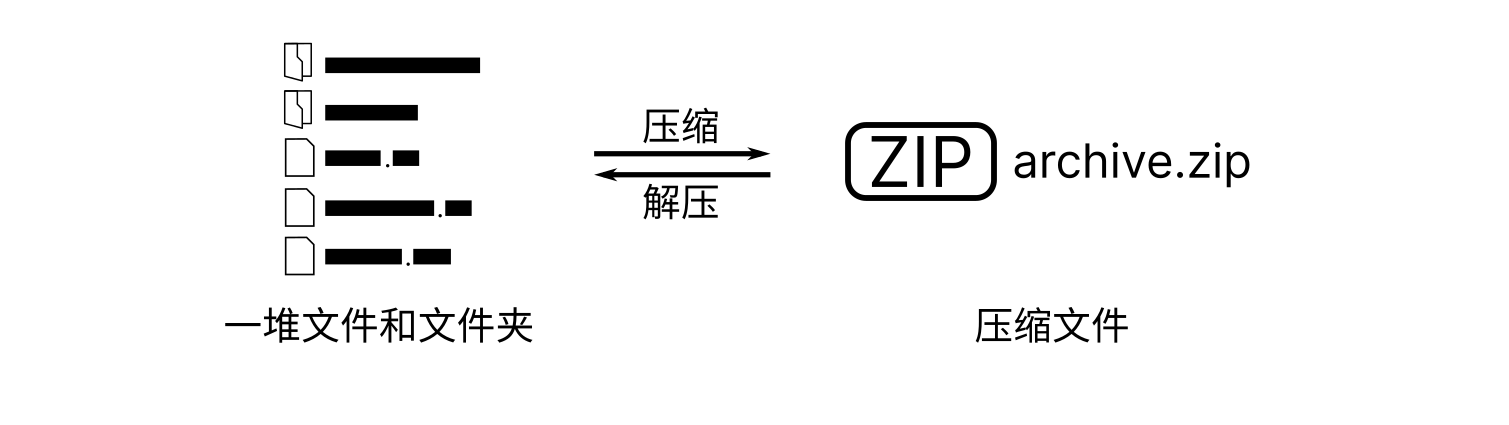
\includegraphics[width=.9\textwidth]{assets/Compress.png}
  \caption{普通文件与压缩文件}
  \label{Compress}
\end{figure}

压缩文件有很多种类。最常用的是 \verb|zip| 文件和 \verb|rar| 文件,但后者的压缩软件是收费的\footnote{具体来说,大多数压缩工具都可以解压 \texttt{rar} 格式的压缩包,但只有 WinRAR 这一款压缩工具可以制作这种格式的压缩包;而这款工具是收费的。详见\nameref{archive-formats-and-tools}。}。
我们建议在与他人交换文件的时候,只使用 \verb|zip| 格式打包。

如果你电脑上已经安装有压缩软件,那么可以参照下面的方法将一批文件打包成一个压缩包:


\begin{itemize}
  \item 选中你要打包的文件。可以是一个文件 / 文件夹,也可以是一群文件 / 文件夹。
  \item 右击,选择【添加到压缩包】或者类似语义的选项。
  \item 设置参数,例如压缩格式(推荐 \verb|zip| 格式)、压缩后的文件的文件名以及压缩方式。\\
    一般来说,压缩后的文件的体积要比原来松散文件的体积小(所谓「压缩」)。
    具体而言,在压缩时可以选择「更快压缩」和「更小体积」之类的选项,前者压缩、解压都更快,但压缩时体积缩小得不明显;后者压缩、解压相对较慢,但压缩后体积可能缩小得更多。
  \item 开始压缩。压缩完成后,在原来的文件的相同目录下,就会生产一个 \verb|<文件名>.zip| 的文件。
\end{itemize}

如果收到一个压缩文件,我们一般需要将它解压。如果你电脑上已经安装有压缩软件,那么可以参照以下方法来解压缩:
右击压缩文件,选择【解压\footnote{部分压缩工具称「解压」为「提取」,是同一个词(Extract)的不同翻译。}到当前文件夹】或者【解压到 \verb|<文件名>\| 】。这两个选项的不同是:

\begin{itemize}
  \item 【解压到当前文件夹】会把压缩文件里的内容直接放在压缩文件的同一目录下。
    例如,如果一个压缩文件 \verb|archive.zip| 里面有 \verb|a.txt| 和 \verb|b.txt| 两个文件,选择此选项,解压后 \verb|a.txt| 和 \verb|b.txt| 都和 \verb|archive.zip| 在同一级目录。 
    \begin{figure}[htb!]
      \centering
      \begin{minipage}{6.2cm}
        \centering
        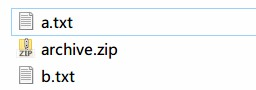
\includegraphics[width=6cm]{assets/Decompress_Current.jpg}
        \caption{【解压到当前文件夹】}
        \label{Decompress_Current}
      \end{minipage}
      \qquad
      \begin{minipage}{6.2cm}
        \centering
        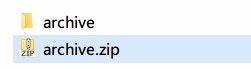
\includegraphics[width=6cm]{assets/Decompress_Sub.jpg}
        \caption{【解压到\texttt{<文件名>\textbackslash}】}
        \label{Decompress_Sub}
      \end{minipage}
    \end{figure}
  \item 【解压到 \verb|<文件名>\| 】会把压缩文件里的内容放在一个子文件夹里面。
    在上面的例子中选择这个选项,会在 \verb|archive.zip| 的同一级目录新建一个文件夹 \verb|archive| ,然后把 \verb|a.txt| 和 \verb|b.txt| 放在 \verb|archive| 文件夹下。
\end{itemize}

我们建议,为了不让自己的工作目录变得混乱,\regcolor{除非你知道自己这样做的原因,否则使用「提取到\texttt{<文件名>\textbackslash}」}。

如果我们只是想查看一个压缩文件的内容,而不把它解压,或者只提取出压缩文件中的一个文件,在系统装有压缩软件的情况下可以直接双击打开压缩文件。
直接双击打开压缩文件,压缩软件会展示出其中的内容。
双击这里面的单个文件可以临时取出这一个文件并打开它,拖拽其中的单个文件到其他地方可以只取出这一个文件而不解压整个压缩文件。

有关压缩格式和压缩软件以及它们的使用的更多细节,请参见\nameref{archive-formats-and-tools}。

\section{文件的打开方式}

在前文中说到,不同类型的文件需要用不同的 app 来打开。
对于一个特定的文件类型,打开它的 app 称为它的「打开方式」。
如果「打开方式」不对,就会出现问题。

容易想到,Word 文档 \verb|doc| 和 \verb|docx| 文件的打开方式就是 Word 软件或者 WPS 软件;图片 \verb|jpg| 、 \verb|jpg| 等的打开方式就是各种看图软件;PDF 文档 \verb|pdf| 的打开方式就是 PDF 阅读器软件,例如 Acrobat 或者 SumatraPDF……

\begin{note}
  可执行文件的打开方式是什么呢?
  这个问题这里不作回答,因为这不构成一个问题。
\end{note}

系统内部维护有一张「表」,这个「表」记录了已知的文件类型(扩展名)和对应的打开方式。
你可以把这张表想象成如表 \ref{regtable} 所示的样子。

\begin{table}[htbp]
  \centering\begin{tabular}{*{3}{>{\small}c}}
    \toprule
    扩展名 & 用什么软件打开 & 软件主程序的路径在哪 \\\midrule
     \verb|txt|   & 记事本 &  \verb|C:\Windows\system32\notepad.exe|  \\
     \verb|docx|  & Word &  \verb|C:\Program Files\Microsoft Office\root\Office16\WINWORD.EXE|  \\
     \verb|mp3|  & 网易云音乐 &  \verb|D:\Program Files (x86)\Netease\CloudMusic\cloudmusic.exe|  \\
    …… & …… & …… \\\bottomrule
  \end{tabular}
  \caption{简易的「表」}
  \label{regtable}
\end{table}

有了这张表,系统就能自动地帮我们选择文件对应的打开方式。
有时,我们不想要用这张表帮我们预置的方式来打开文件。
比如,打开 \verb|jpg| 图片的默认方式是「图片」软件,但如果我们想\regcolor{暂时}用「Photoshop」来打开它,我们可以这样做:

\begin{itemize}
  \item 右键要打开的这个 \verb|jpg| 文件,选择【打开方式】,在里面选择【Adobe Photoshop】。
    \begin{figure}[htb!]
      \centering
      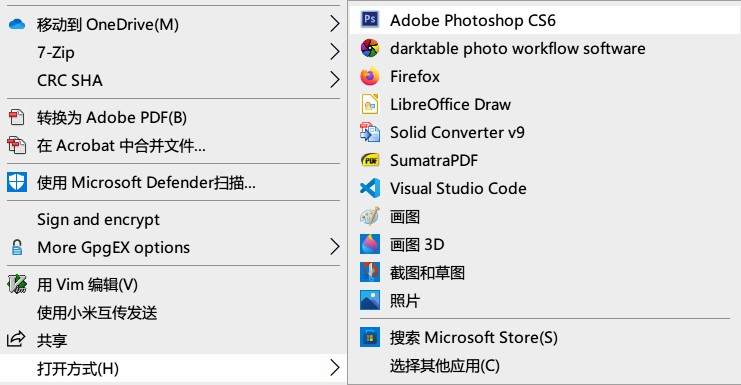
\includegraphics[width=9cm]{assets/Select_Open_with.jpg}
      \caption{更改打开方式}
      \label{Select_Open_with}
    \end{figure}
  \item 如果上一步找不到「Adobe Photoshop」,那么选择【打开方式】→【选择其他应用】。
    然后在弹出的对话框中寻找【Adobe Photoshop】,点击并选择【确定】。
    注意\regcolor{不要}勾选「始终使用此应用打开 \verb|.jpg| 文件」。
    \begin{figure}[htb!]
      \centering
      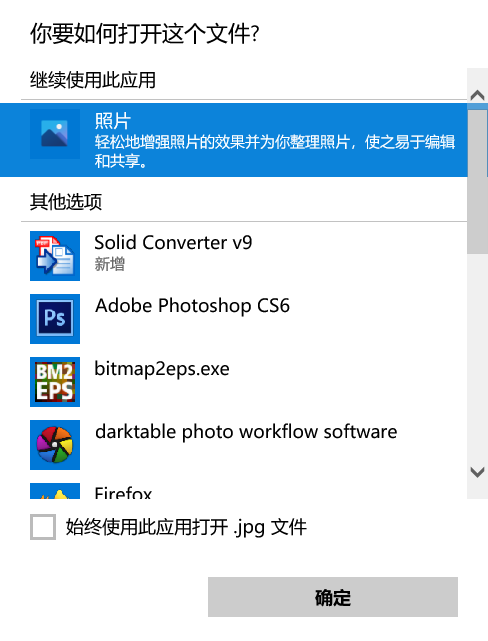
\includegraphics[width=5cm]{assets/Open_with.png}
      \caption{进一步选择}
      \label{Open_with}
    \end{figure}
  \item 如果上一步还找不到「Adobe Photoshop」,而你确实电脑上装有 Photoshop,那么可能需要手动找到 Photoshop 的那个可执行文件,也就是它的 \verb|exe| 文件。
    这个文件的路径——也就是软件的安装路径——在下一章我们会提到。
    一般来说是在 \verb|C:\Program Files| 或者 \verb|C:\Program Files (x86)| 之下的某个文件夹中。
\end{itemize}

\regcolor{如果你想永久地指派某一文件的打开方式,则可以在上面步骤的基础上,勾选【始终使用此应用打开 \texttt{xxx} 文件】。}
这样,系统内部的那张「表」就会被更改,系统以后都会用你指派的新应用来打开这种文件。

除了你手动更改之外,这张「表」还可能在这些情况被更改:

\begin{itemize}
  \item 系统安装更新,即 Windows Update 之后,这张表可能会被重置而丢失一些项目,造成某些文件突然无法打开。这往往是由于你使用的对应软件并不是原版,而是某种「精简版」所造成的。
  \item 新安装一个软件时,软件安装程序可能写入新的表项,来为即将安装的新软件的文件类型配置打开方式。
  \item Windows 的各种恶性 bug 和恶心操作。例如,Windows 会时不时用 Microsoft Edge 代替其他软件来打开网页文件和 \verb|pdf| 文件等。\CJKsout*{(微软你坏事做尽)}
\end{itemize}

如果你的文件关联某天突然失效,即某种类型的文件突然无法打开,但对应的软件工作正常,那么可以考虑是否是上面的原因。

\section{管理好你的文件}

管理好我们的文件,不外乎两个方面:

\begin{itemize}
  \item 对自己的文件进行整理归类。比起将所有文件「随手乱放」,如果我们将自己的文件按它们的性质、类别等归类存放,必然有助于提升我们的工作效率。
  \item 不把(重要)文件放在 C 盘。在前文我们说了,C 盘是 Windows 系统整个所在的地方。
    尽管发生这种情况的概率很低,但当我们的电脑因为这样或那样的原因损坏,而需要重装系统的时候,你会不得不失去 C 盘的所有文件——安装系统的第一步就是格式化 C 盘。
    让自己的文件远离 C 盘,是合理管理我们的文件的重要部分。
\end{itemize}

\subsection{为文件安家}

首先为你要放的文件选择一个合适的位置。

桌面,以及 Windows 系统预置的那些文件夹(「文档」「视频」「图片」等,打开【此电脑】就可以直接看到),除非按照后文所介绍的方法更改位置,否则全部是 C 盘内部的空间,因此在你手动更改它们的位置之前,\regcolor{不建议}将自己的文件放在这些地方。

另一方面,非 C 盘的分区,例如 D 盘甚至后续更多的磁盘分区,都是可以考虑的存放自己资料的位置。

找到一个合适的位置后,我们便可以建立一套自己的分类方法来对文件进行整理和分类。


\begin{itemize}
  \item 例如你有一些「学习资源」,你便可以在 D 盘或是什么别的盘建立一个名为「学习资源」的文件夹,再在其下——无论是按学科(例如「高数」「线代」「物理」),还是按时间(例如「大一上」「大一下」)——建立更多的子文件夹,来为它们进行更为详尽的分类。
  \item 再例如你有许多「大片」,你也可以按照地区、上映时间甚至是主演什么的为它们分类。
    不过鉴于大片不仅是名气大,占用空间也大,我们推荐腾出一个分区(甚至是一块硬盘)来存放它们。
\end{itemize}

总的来说,\regcolor{「为你的文件进行合理分类」}与\regcolor{「将你的硬盘进行合理分配」}便是这里的核心思想。

\subsection{定期打扫}

电脑里面的东西总是随着我们的日常使用而越积越多 \CJKsout*{(这里点名 QQ 的 \texttt{FileRecv} 和 \texttt{Image} 文件夹,藏得又深,又乱七八糟;还有微软的更新,一更一大堆)},所以定期检查你不需要的东西然后扔掉它们显得尤为重要。

对于系统分区 C 盘来说,你不去动它,它也会被塞入一些诸如系统临时文件、Windows 更新文件等等这些。
我们推荐新手用户们运用一些诸如「火绒安全软件」「360 电脑管家」之类的 app 中的清理功能进行文件的清理。

但是上述软件并不会把我们日常中积累的用户文件(例如你收到的课件、文档等)也清理掉,但在日常使用过程中,我们也会不可避免地产生许许多多的冗余文件,或是曾经需要而现在不再需要的文件。
这里不妨就来看看上文所讲的那个 \verb|FileRecv| 文件夹:

\begin{itemize}
  \item 这个文件夹默认位于 \verb|文档\Tencent Files\<QQ 号>\| 处,每个不同的 QQ 号都有一个属于自己的个人文件夹。
    如果你没有按照后文「更改用户文件夹的存储位置」迁移「文档」文件夹的话,这东西也在 C 盘里,因为「文档」是在 C 盘里的;
  \item 点开 \verb|FileRecv| ,你在使用 QQ 的过程中接收到的所有文件都在此处,其中通过手机发给电脑的文件存储于专属子文件夹 \verb|MobileFile| 中;
  \item 将 \verb|FileRecv| 文件夹中的所有文件检查一遍,有用的就如上文所述归类、无用的则直接删除,这就大功告成了。
\end{itemize}

事实上 QQ 为用户提供了更改用户个人文件夹位置的功能,但是似乎更改的时候并不会将你曾经接收的文件一并移走,着实不好用,这里并不推荐。

同样地,在你已经归好类的文件体系中,也要时不时进行检查,删去冗余与无用文件,这样能够保持你的文件系统简而精。
《礼记·大学》载:「苟日新,日日新,又日新。」如是而已。

\subsection{更改用户文件夹的存储位置 *}

上文提到了一个叫做 \verb|文档| 的文件夹,它是系统预置的一个用户文件夹。
在介绍这一部分之前,我们先简单提一下「用户文件夹」是什么。

\begin{figure}[htb!]
  \centering
  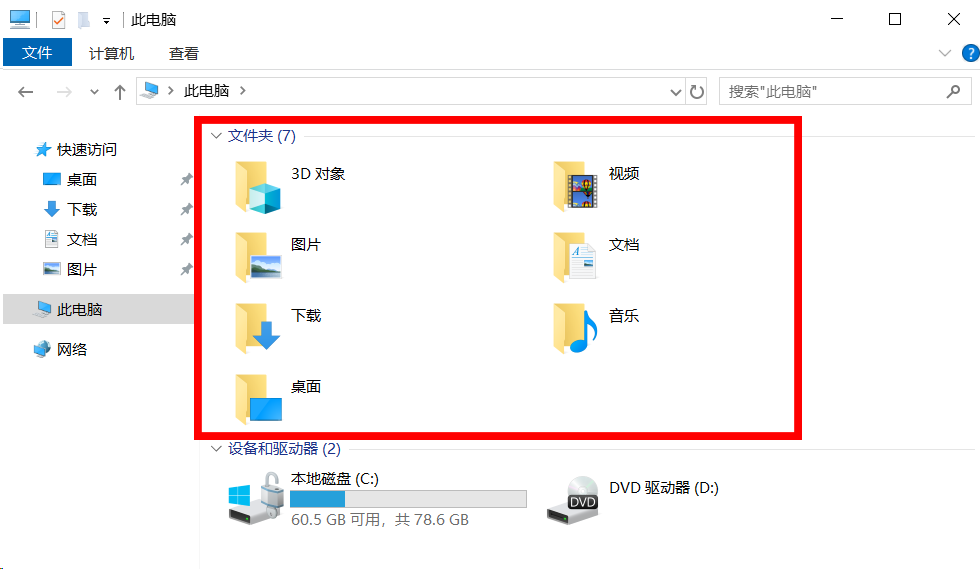
\includegraphics[width=11cm]{assets/User_directories.png}
  \caption{用户文件夹}
  \label{User_directories}
\end{figure}

如前所言,Windows 系统默认为用户准备了几个文件夹来进行文件的分类。
通过双击桌面上的【此电脑】,展开【文件夹】折叠项,这些文件夹就如图 \ref{User_directories} 所示。

Windows 系统的本意,是希望用户可以借助这些文件夹来辅助进行文件的整理。
可是,这些文件夹默认情况下全部位于 C 盘(路径是 \verb|C:\用户\<你的用户名>\| ),而把大量的个人文件放在 C 盘是我们所不建议的。
那这些系统「好心」准备给我们的文件夹就都不能使用了吗?
答案是否定的——通过迁移这些文件夹到 D 盘,我们可以在利用好这些用户文件夹的同时,保证自己的数据安全和系统稳定。

\begin{note}
  看到这几个文件夹中的「桌面」,你是否会有点奇怪?桌面为什么也是这里的一部分呢?
  事实上,桌面的本质也是一个用户文件夹。桌面上你放的文件、各个 app 的快捷方式都在这个文件夹中。
\end{note}

我们打开 \verb|C:\用户\<你的用户名>\| 可以看到全部的用户文件夹。
这些文件夹涵盖了「桌面」「文档」「图片」「音乐」「视频」等多种类别,并且都配有形象的图标,如图:

\begin{figure}[htb!]
  \centering
  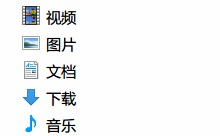
\includegraphics[width=4cm]{assets/All_User_Directories.jpg}
  \caption{更多用户文件夹}
  \label{All_User_Directories}
\end{figure}

我们的目的是把这些文件夹「迁移」到 D 盘(或者其他的某个磁盘,这里以 D 盘为例)。
这样,我们就可以充分地利用系统预置的这一批用户文件夹了。

右击某个我们想要迁移的文件夹(比如【桌面】),选择【属性】,然后切换到【位置】选项卡,如图:

\begin{figure}[htb!]
  \centering
  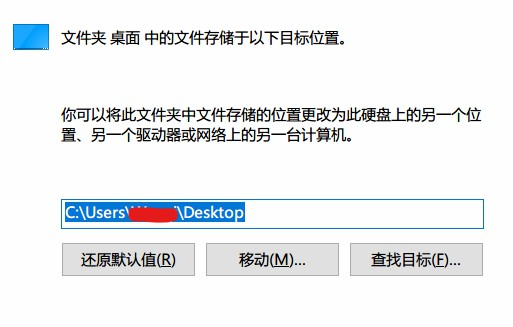
\includegraphics[width=8cm]{assets/Change_Directories.jpg}
  \caption{更改用户文件夹位置}
  \label{Change_Directories}
\end{figure}

我们将这里文本框中

\begin{verbatim}
  C:\Users\<你的用户名>\
\end{verbatim}

这一部分\regcolor{(注意:最后一个\texttt{Desktop}、\texttt{Documents}之类的名字不要动!)}\footnote{如果你不小心把一个用户文件夹的位置设置成了某个磁盘的根目录(比如说\texttt{D:\textbackslash}),会触发 Windows 系统的一个 bug,导致很难再改回来。\CJKsout*{(辣鸡 Windows)}}改成

\begin{verbatim}
  D:\
\end{verbatim}

\regcolor{也就是说,对于「桌面」而言,改完之后的完整路径是}

\begin{verbatim}
  D:\Desktop
\end{verbatim}

例如:

\begin{figure}[htb!]
  \centering
  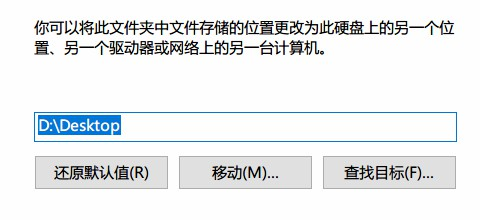
\includegraphics[width=8cm]{assets/Destination.jpg}
  \caption{填入目标位置}
  \label{Destination}
\end{figure}

点击【应用】,提示「文件夹 ‘D:\textbackslash{}Desktop’ 不存在,是否新建该文件夹」,选择【是】。

紧接着提示「是否要将所有文件从原位置移动到新位置」,选择【是】。

一般来说移动操作很快就会完成。完成后,点击【确定】。
这样「桌面」文件夹就被成功地迁移到了 D 盘。
你可以打开 \verb|D:\桌面| 来查看其中的内容,与你桌面上真正看到的东西应该大同小异。

\begin{note}
  对于桌面而言,现在你放在桌面上的文件本质上就存在 D 盘里了。
  但我们依然不建议你在桌面上放太多文件——因为这样不方便你自己寻找。
\end{note}

\regcolor{强烈建议进行迁移的用户文件夹有:}\regcolor{「文档」「桌面」「下载」。}

\regcolor{建议进行迁移的用户文件夹有:}\regcolor{「视频」「图片」「音乐」。}

迁移完成之后,你可以在迁移之后的位置(比如 D 盘)看到这些文件夹。
它们现在不在原来的 \verb|C:\用户\<你的用户名>\| 那里了。

\begin{figure}[htb!]
  \centering
  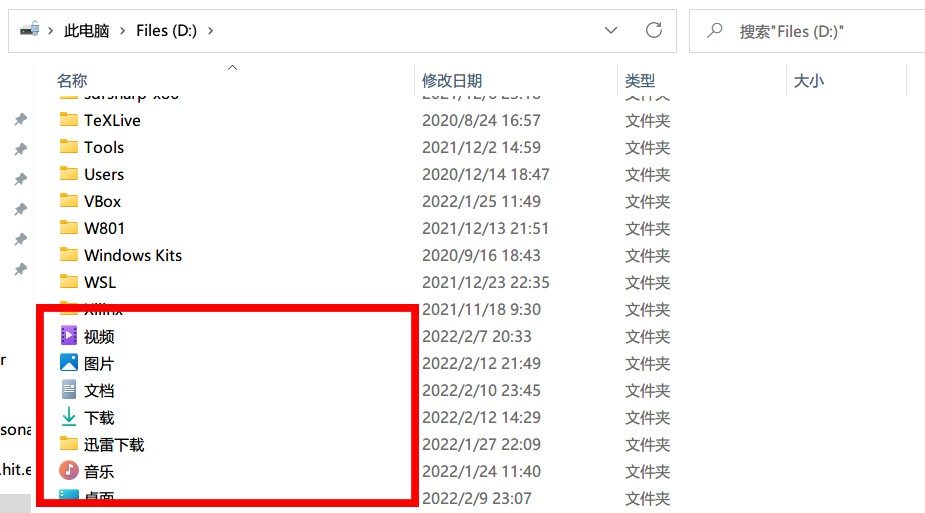
\includegraphics[width=12cm]{assets/Moved_user_directories.jpg}
  \caption{新的用户文件夹位置}
  \label{Moved_user_directories}
\end{figure}

\practice

\begin{enumerate}
  \item 查看自己电脑的几个分区的「卷标」,并依照自己的文件分类习惯修改成自己所喜欢的名字。例如,叫「资料」或者「Files」就比「新加卷」或者没有卷标(会显示「本地磁盘」)要直观得多。
  \item 尝试把一个图片文件的扩展名改成 \verb|txt| ,然后用「记事本」打开它。你看到了什么?\textit{记得改回来哦!}
  \item 试着迁移用户文件夹到 D 盘或者其他非 C 盘的分区,然后利用这些用户文件夹帮助自己整理文件。\\
    注意迁移的时候千万看清楚目标路径是完整的 \verb|D:\Documents| 、 \verb|D:\Desktop| 这样的路径,而不是光秃秃的一个 \verb|D:\| 。
  \item 整理你的 QQ 文件接收文件夹 \verb|FileRecv| 。
  \item 选择你自己的几个文件和文件夹,把它们打包成一个压缩文件 \verb|MyArchive.zip| ,复制到其他的某个地方,尝试两种不同的解压方式「提取到当前位置」「提取到 MyArchive\textbackslash{}」。
  \item 创建一个文档(可以是纯文本文件 \verb|txt| 或者 Word 文档 \verb|docx| 等)并写入一些内容,然后制作它的两个快捷方式,并把这两个快捷方式放在两个与源文件都不一样的地方。试着双击打开那两个快捷方式,你发现了什么?删掉两个快捷方式中的一个,源文件被删除了吗?
    另一个快捷方式还在吗?
\end{enumerate}